\chapter*{Úvod}
\phantomsection
\addcontentsline{toc}{chapter}{Úvod}


Osazovací automaty pro povrchovou montáž, též známe pod názvem pick and place (PnP), jsou stroje sloužící na osazování desek plošných spojů SMD součástkami. Hrají tak nedílnou součást v celém procesu výroby elektronických zařízení. 
Na výrobních linkách pro sériovou výrobu mají svoje místo již desetiletí. Na druhou stranu v mlosériové výrobě (jednotky kusů) a prototypové výrobě se s nimi skrz jejich vysokou pořizovací cenu setkáváme zřídkakdy.
Osazování DPS lze poptat také jako službu, která je již cenově dostupnější. Pro prototypovou výrobu to ale naráží na fakt, že dodavatelé těchto služeb vyžadují součástky ve strojově zpracovatelné formě. Tedy na rolích, platech a v tubách. V prototypové a malosériové výrobě se ale pracuje spíše se střiženými  páskami a jednotlivými součástkami.


V posledních letech se čím dál častěji setkáváme s fenoménem Open Source Hardware. Je to filozofie tvorby hardware a jeho sdílení včetně všech zdrojových souborů s komunitou. Tedy jakási obdoba známého Open Source Software.

\begin{figure}[h!]

  \centering
    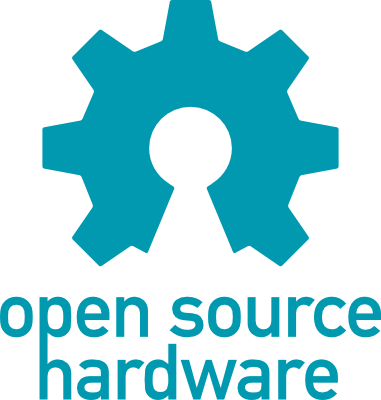
\includegraphics[width=0.4\linewidth]{obrazky/openhw.png}%
    \caption{Open Source Hardware.}
\end{figure}

Vzhldem k mojí potřebě častého prototypování a přispívání právě k Open hardware je cenově dostupný osazovací automat velice žádaný. Jak plyne se zadání, cílem této diplomové práce je tedy kompletní tvorba vlastního osazovacího automatu na SMD součástky za dostupnou cenou. Jedná se tak o komplexní projekt vyžadující schopnosti od návrhu mechanické konstukce, elektroniky a řídícího software.

 Celá práce je vedena v duchu opensource a open hardware, všechny části projektu včetně zdrojových kódů jsou tak volně dostupné na internetu pro širokou veřejnost.
